
%(BEGIN_QUESTION)
% Copyright 2006, Tony R. Kuphaldt, released under the Creative Commons Attribution License (v 1.0)
% This means you may do almost anything with this work of mine, so long as you give me proper credit
Et rør fylt med vann til 2 meter vinkles 40$^{\circ}$ fra horisontalplanet. Regn ut det hydrostatiske trykket som manometeret vil vise i pascal.

$$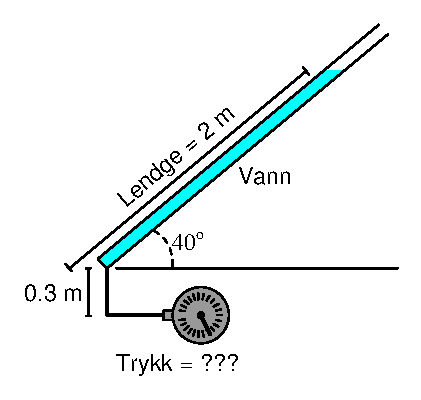
\includegraphics[width=7cm]{i00234x01.eps}$$

\underbar{file i00234}
%(END_QUESTION)





%(BEGIN_ANSWER)

\noindent
{\bf Delvis svar:}

\vskip 10pt

Det som teller her er den {\it vertikale} høyden på vannsøylen, ikke den skrå lengden.  Dette er i praksis et trigonometriproblem: finn lengden på siden motstående 40$^{o}$-vinkelen, gitt hypotenusen på 10 fot (120 tommer).

$=\Delta P = 15554$ Pa
%(END_ANSWER)





%(BEGIN_NOTES)

Motstående side = (120 in)(sin 40$^{o}$) = 77.13 "W.C.

\vskip 10pt

Dette hydrostatiske trykket tilsvarer 2.787 PSI.  Konvertert til PSIA får vi 17.49 PSI.  Konvertert til atmosfærer får vi 1.19 atm.


%INDEX% Physics, static fluids: hydrostatic pressure

%(END_NOTES)
